\section {PROGRAMS}

Tab \textit{Programs} is used to configure sequence of operations possess parameterized actions which can be using to automation control of machine. User create program which consist sequence of operation named as subprogram. Subprogram possess parametrization operations as stages

	\begin{figure}[!h] 
	\centering 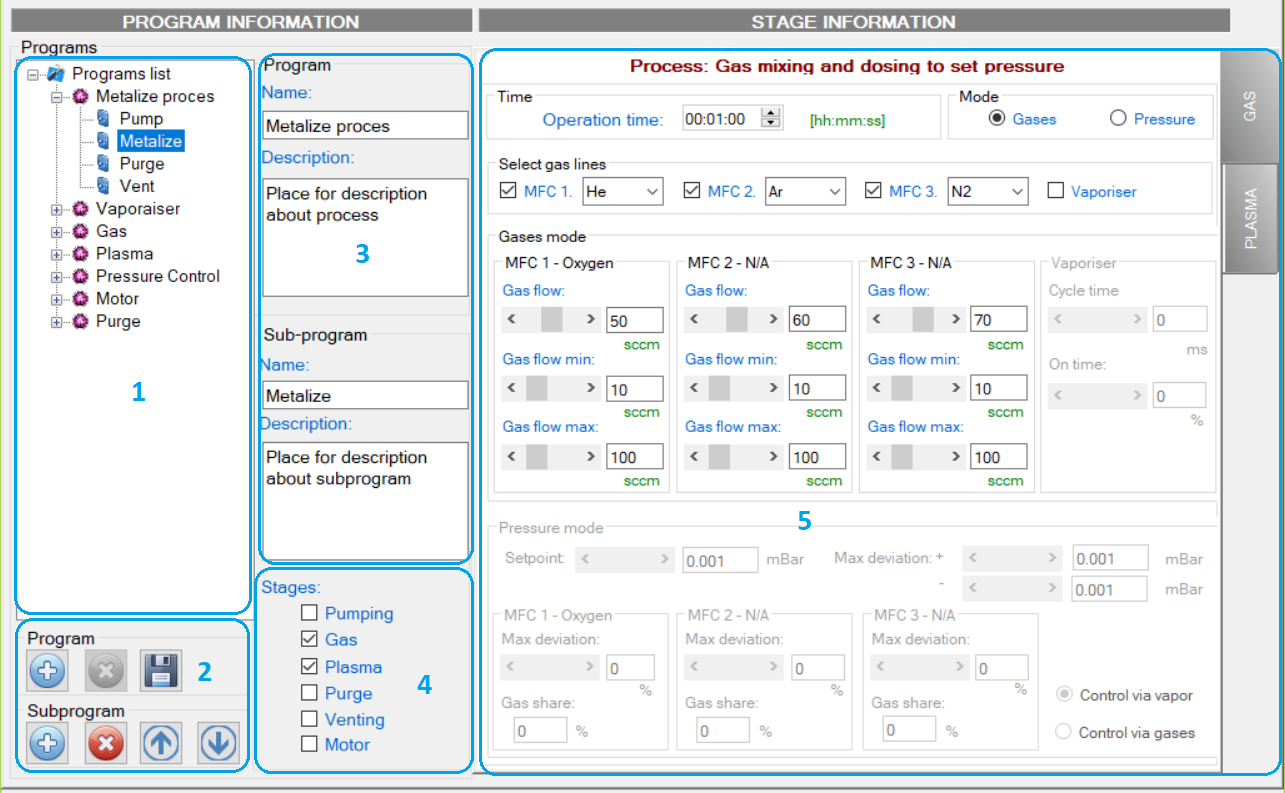
\includegraphics[width=0.8\textwidth]{Graphic/Programs/ProgramsTab.png}	
	\caption{Tab main screen}
	\label{tab_main_screen}
	\end{figure}
	\FloatBarrier

Tab was divided  on five section:

\begin{enumerate}
	\item List of  configured  programs 
	\item Group of buttons which allow to on add/remove program/subprogram and move subprogram within a program
	\item Description of program and subprogram
	\item Selected stages which are included to subprogram
	\item Parameters of selected stage of subprogram
\end{enumerate}

Each subprogram can consist one or several stages listed below:
\begin{itemize}
	\item Pumping
	\item Gas
	\item Plasma
	\item Purge
	\item Motor
\end{itemize}

\subsection{Pumping}

Stage \textit {Pumping} give us possibility in easy way to pumped a chamber. We should only specify setpoint of pressure and maximum time to achieve this setpoint.

	\begin{figure}[!h] 
	\centering 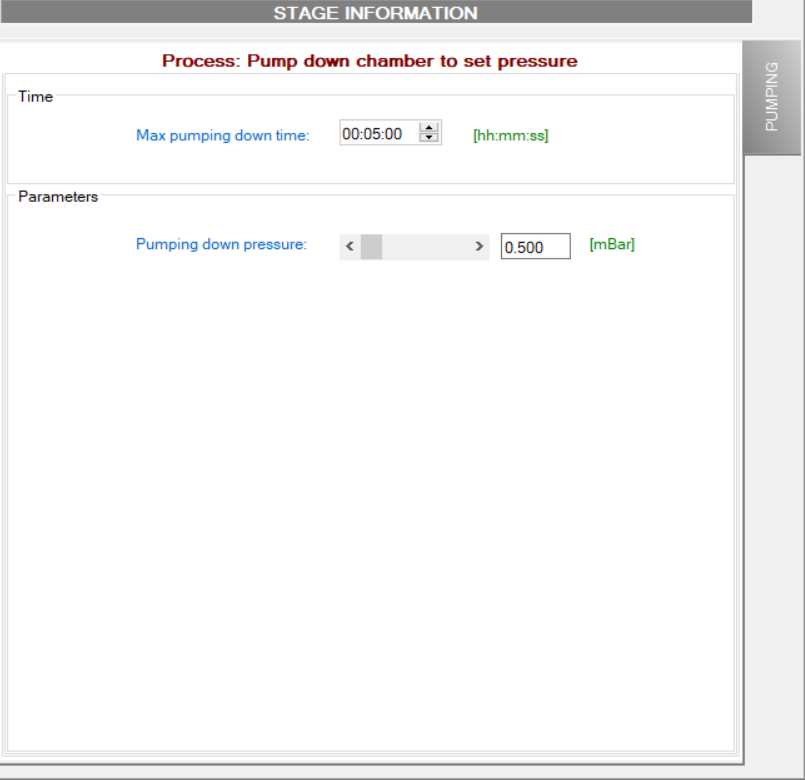
\includegraphics[width=0.7\textwidth]{Graphic/Programs/Pumping.png}	
	\caption{Stage Pumping}
	\label{stage_pumping}
	\end{figure}
	\FloatBarrier

Procedur \textit{Pumping} at first make pumping line from fore pump to valve SV. When time was achived, valve SV will be opened and chamber will be pumped. Time to pump line from fore pump to SV is setting in \textit{Service} tab section \textit{Pump}. When chamber not achived setpoint of pressure in defined  time, stage will be reported an error and subprogram will be emergency stopped.


\subsection{Gas}

Stage \textit{Gas} is  responsible on dosing gases to chamber. Gas can be dozing to chamber in one of two mode:

\begin{itemize}
	\item Gases
	\item Pressure
\end{itemize}
When we selected corresponding gas mode we should decide which mass flow controller should be responsible for inject gas to chamber.

\subsubsection{Gases}

Mode \textit{Gases} allow us on set setpoint of flow for mass flow controller and specify range of flow what should be. Flow range is parametrized by settings \textit{Gas flow min} and \textit{Gas flow max}.  When flow is out of range procedure will be reported error and subprogram will be emergency stopped. 

	\begin{figure}[!h] 
	\centering 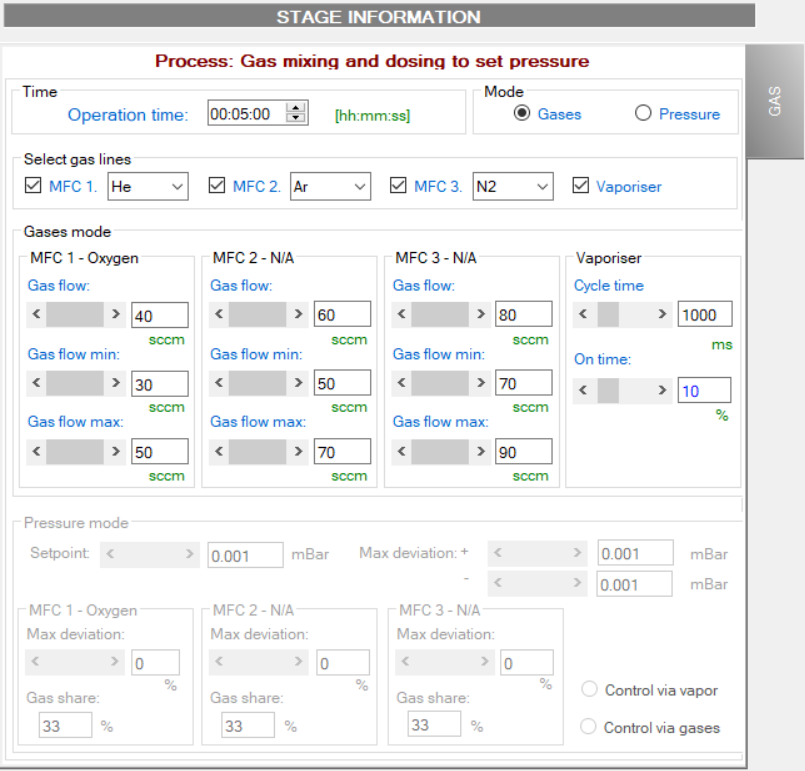
\includegraphics[width=0.7\textwidth]{Graphic/Programs/Gas_ModeGas.png}	
	\caption{Stage Gas - mode Gasses}
	\label{stage_gas_ mode_gasses}
	\end{figure}
	\FloatBarrier

Work of vaporaiser is specified by cycle time or count of short shots gas injection. When vaporiser work in \textit{Cycle} mode we defined percentage of fulfillment thats mean how long in period of one cycle, vaporiser should be open. When vaporizer work in \textit{Dosing} mode we specify count of shots per minute which inject gas to chamber 

\subsubsection{Pressure}

In pressure mode level of gas flow in chamber is set automatically. We only specify setpoint of pressure which should be hold in chamber and allowed deviation.  Pressure can be held in chamber based on dosing gas from:

\begin{itemize}
	\item MFC
	\item Vaporaiser 
\end{itemize} 

When we want using gases from MFC we should select option \textit{Control via gases}. In this mode we specify percentage share of flow for corresponding MFC. Sum share percentage flow of all MFC is 100\%.  We also can defined maximum deviation from setpoint of flow for each MFC. \\

When we want using gas from vaporaiser we should select option \textit{Control via vapor} then pressure in chambre will be held via vaporaiser


	\begin{figure}[!h] 
	\centering 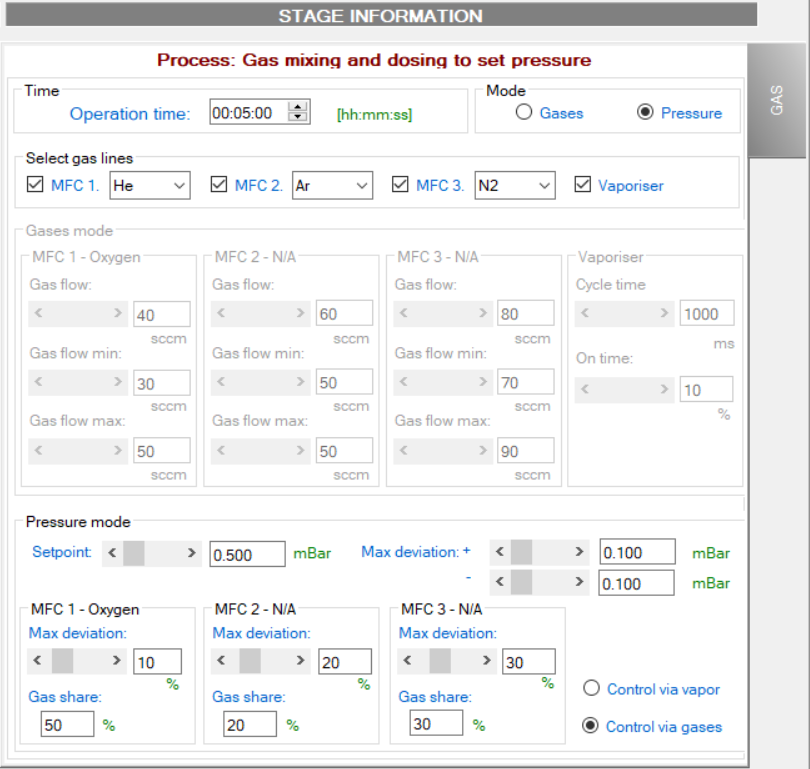
\includegraphics[width=0.64\textwidth]{Graphic/Programs/Gas_ModePressure.png}	
	\caption{Stage Gas - mode Pressure}
	\label{stage_gas_ mode_pressure}
	\end{figure}
	\FloatBarrier

\subsection{Plasma}

Stage \textit{Plasma} give us possibility to control of power supply in order to achieve plasma in chamber.

	\begin{figure}[!h] 
	\centering 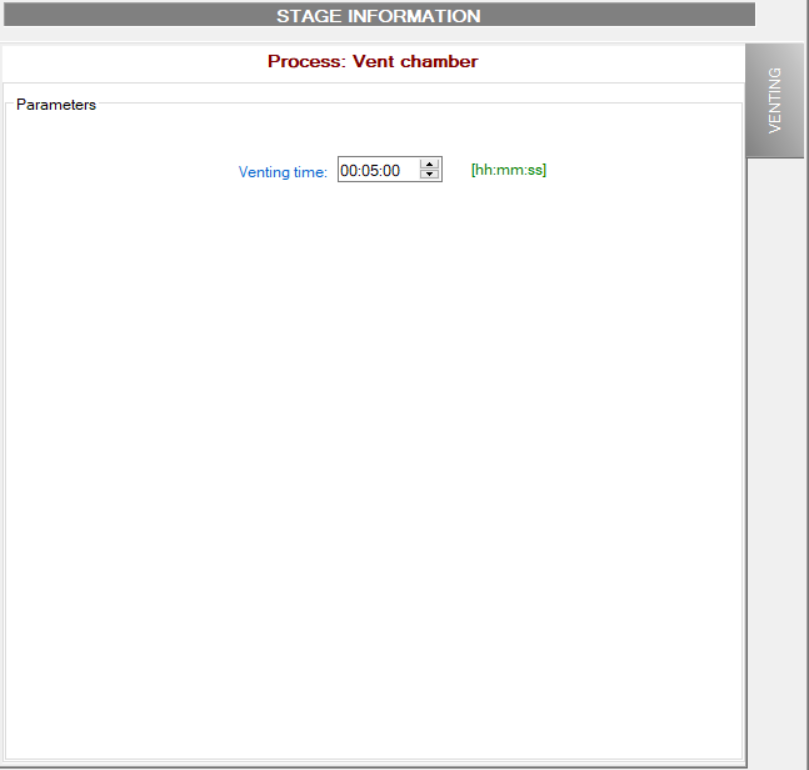
\includegraphics[width=0.64\textwidth]{Graphic/Programs/Venting.png}	
	\caption{Stage Plasma}
	\label{vent_purge}
	\end{figure}
	\FloatBarrier

Work of power supply is controlled by two parameters: range of time when power supply is running and percent  setpoint of it power .

\subsection{Purge}

Stage \textit{Purge} allow us to purging of chamber from unnecessary gases

	\begin{figure}[!h] 
	\centering 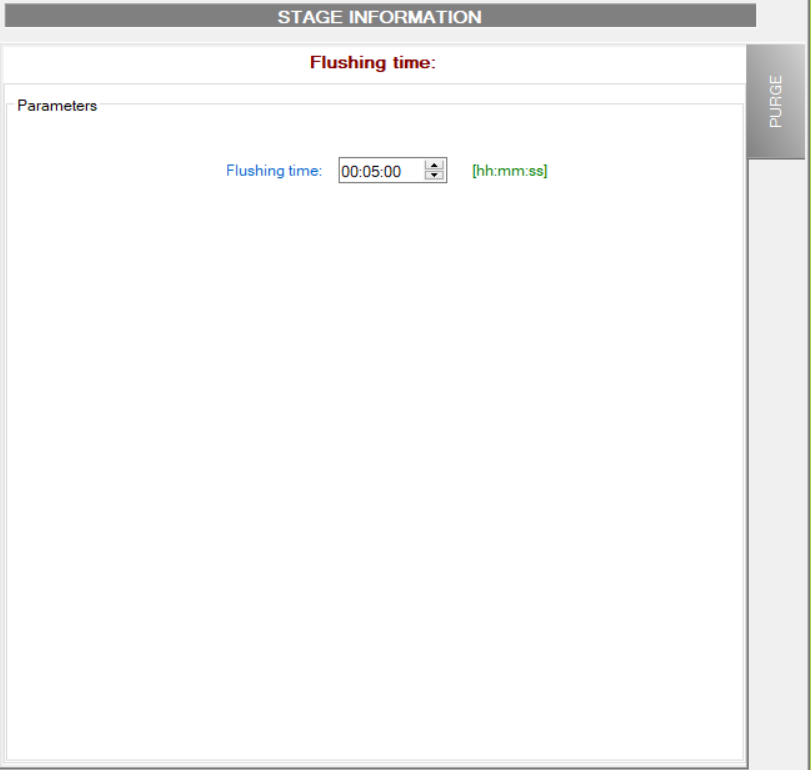
\includegraphics[width=0.7\textwidth]{Graphic/Programs/Purge.png}	
	\caption{Stage Purge}
	\label{stage_purge}
	\end{figure}
	\FloatBarrier

Procedure \textit{Purge} opening purge valve on defined period time. When setting time will be achieved, valve will be closed and procedure will be completed. 

\subsection{Venting}

Stage \textit{Venting} allow us to vented of chamber.

	\begin{figure}[!h] 
	\centering 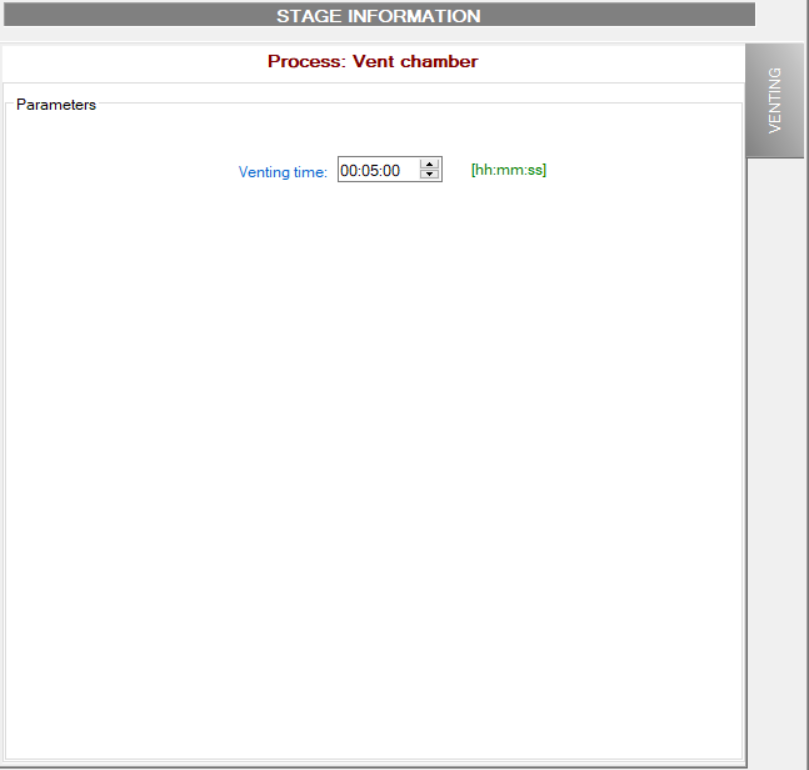
\includegraphics[width=0.7\textwidth]{Graphic/Programs/Venting.png}	
	\caption{Stage Vent}
	\label{stage_vent}
	\end{figure}
	\FloatBarrier

Procedure \textit{Venting} opening vent valve on defined period time. When setting time will be achieved, valve will be closed and procedure will be completed. 

\subsection{Motor}

Stage \textit{Motor} give us posibility to control move of motor.

	\begin{figure}[!h] 
	\centering 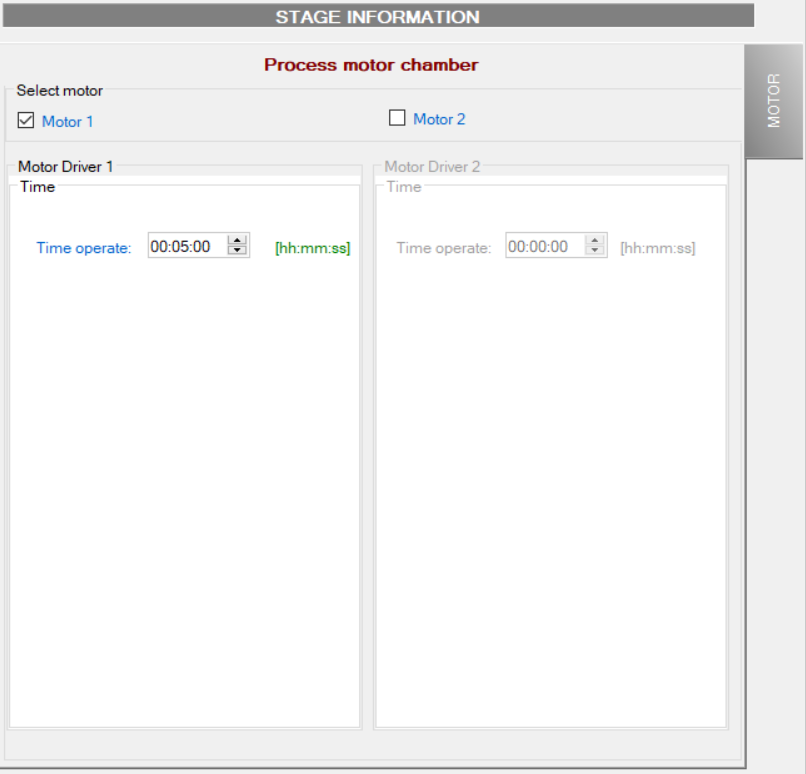
\includegraphics[width=0.7\textwidth]{Graphic/Programs/Motor.png}	
	\caption{Stage Motor}
	\label{stage_motor}
	\end{figure}
	\FloatBarrier

Procedure turn on motor and after specified time motor will be turned off. We can choose motor which should be controlled.

